\clearpage
\visHeader

\subsection{A first look at EA}

\begin{itemize}
\FloatBarrier
\hypertarget{simpleDemo vis}{}
\item[$\blacktriangleright$] Can you locate the new \texttt{Demo.eap} file in your package explorer? This is the EA project file you'll be
modelling in. Don't worry about any other folders at the moment - all problems will be resolved by the end of this section.

In the meantime, do not rename, move, or delete anything.

\item[$\blacktriangleright$] Double-click \texttt{Demo.eap} to start EA, and choose \texttt{Ultimate} when starting EA for the first time.

\item[$\blacktriangleright$] In EA, navigate to ``Extensions/MOFLON::Ecore Addin/Validate All'' (Fig.~\ref{ea:validate_dropdown}). Not only will this check
your diagram for errors, it will export your files to your Eclipse workspace once it's successful.

\begin{figure}[htbp]
	\centering
  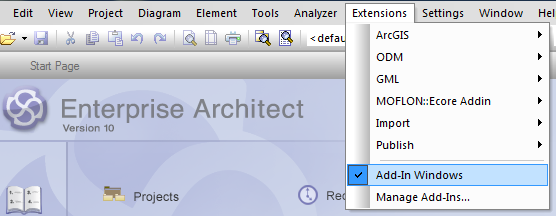
\includegraphics[width=0.8\textwidth]{ea_extensionMenu}
	\caption{Export from EA} 
	\label{ea:validate_dropdown} 
\end{figure}

\item[$\blacktriangleright$] Please note that this submenu is limited, and does not provide access to all eMoflon functionality. You can activate eMoflon's full
control panel by enabling ``Extensions/Add-In Windows'' (Fig.~\ref{ea:validate_dropdown}). To export from here, click \texttt{All} in the ``Validate''
section (Fig.~\ref{ea:controlPanel})


\begin{figure}[htbp]
	\centering
  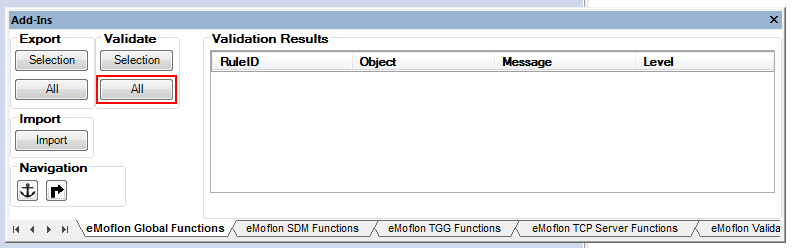
\includegraphics[width=0.9\textwidth]{ea_controlPanelValidateAll}
	\caption{eMoflon's control panel} 
	\label{ea:controlPanel} 
\end{figure}

\item[$\blacktriangleright$] Now try exploring the EA project browser! Try to navigate to the packages, classes, and diagrams. Don't worry if you don't
understand that much - we'll get to explaining everything in a moment. Just make sure not to change anything!

\item[$\blacktriangleright$] Switch back to Eclipse, choose your metamodel project, and press F5 to refresh. A new folder should appear, and your errors should
disappear after a few seconds. Since you've chosen to use our visual syntax, there isn't much to look at here. The export from EA places all required files in a
hidden folder (.temp) in the project, and refreshing triggers a build process that invokes our code generator automatically. 

\item[$\blacktriangleright$] You should be able to monitor the progress with the green bar in the lower right corner (Fig.~\ref{eclipse:build}). Pressing the
symbol opens a monitor view that gives more details of the build process. You don't need to worry about any of these details, just remember to refresh your
Eclipse workspace after an export.

\jumpSingle{validate common}

\vspace{0.5cm}

\begin{figure}[htbp]
	\centering
  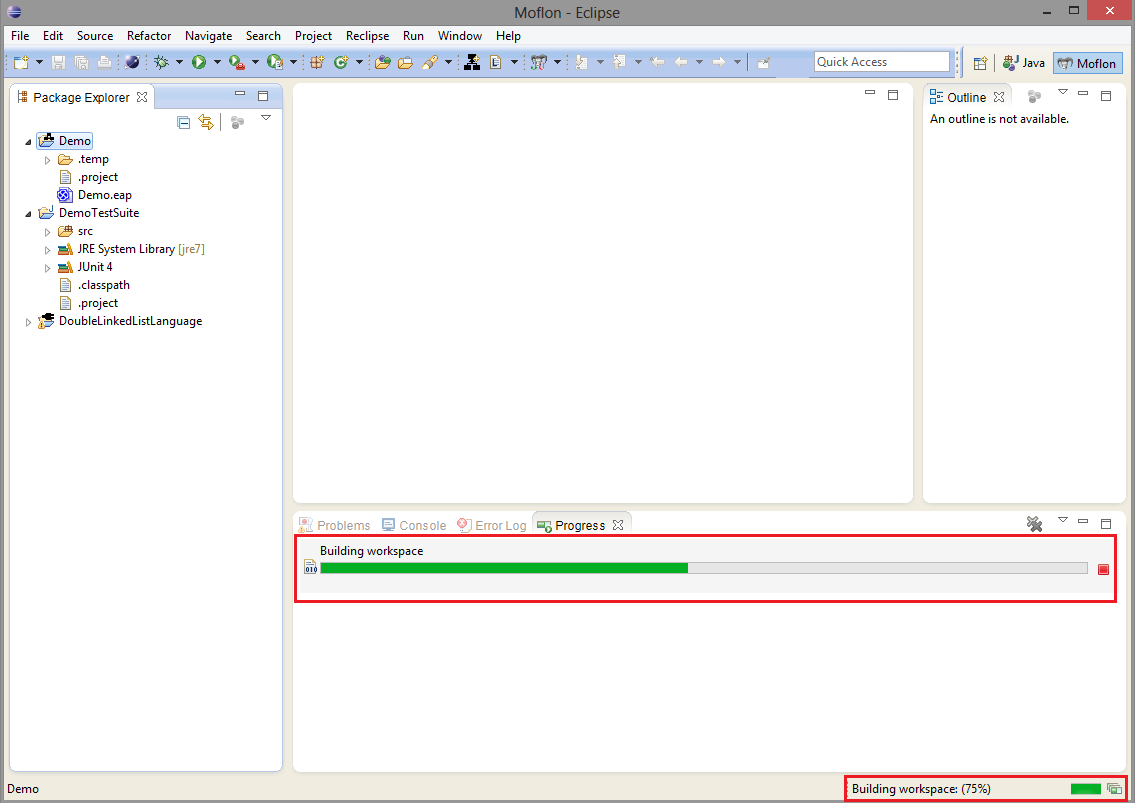
\includegraphics[width=0.9\textwidth]{eclipse_buildingProgress}
	\caption{Eclipse workspace when using visual syntax} 
	\label{eclipse:build} 
\end{figure}

\vspace{0.5cm}

\item[$\blacktriangleright$] If you're ever worried about forgetting to refresh your workspace, or if you just don't want to bother with having to do this,
Eclipse does offer an option to do it for you automatically. To activate this, go to ``Window/Preferences/General/Workspace" and select \texttt{refresh on
access}.

\end{itemize}